%% --------------------------------------------------------------------
\section{Empirical Evaluation}
\label{sec.evaluation}
%% --------------------------------------------------------------------

\begin{table}[!t]
  \caption{Genetic Algorithm Configurations}
  \label{tbl.gen.config}
  \scriptsize
  \centering
  \begin{tabular}{l|r|r|r}
    \toprule
    \textbf{Parameter Name} &$\Random$&$\Genetic$ &$\RGenetic$ \\
    \hline
    Population size                   & 50  & 50  & 50  \\
    Archive size                      & 1   & 25  & 25  \\
    Maximum number of generations     & 200 & 200 & 200 \\
    Crossover rate                    & 0   & 0.5 & 0.5 \\
    Mutation rate                     & 0   & 0.5 & 0.5 \\
    History window size               & -   & -   & 10  \\
    \bottomrule
  \end{tabular}
\end{table}

In order to evaluate the feasibility of our test framework, we conducted an empirical study on a set of subjects (see Section~\ref{sub.sec.case.studies}). All experiments were submitted as a batch mode job on a cluster machine with 32 HT Cores and 256 GB RAM running under Scientific Linux 7.3. We have created three different instances of the JS testing framework --- each one is based on a slight variation of the underlying GA. The first version, which plays the role of our baseline, is \emph{Random} ($\Random$). Instead of applying crossover and mutation to evolve the population, this algorithm regenerates the new population randomly from scratch. It is important to note  that the random version also benefits from both preliminary static analysis and dynamic constant propagation as part of the fitness evaluation. The second version is \emph{Genetic}~($\Genetic$) --- it literally follows all of the steps prescribed by the genetic framework in Figure~\ref{fig.framework.architect}. The last version is \emph{Genetic with Restart} ($\RGenetic$). It is based on Algorithm~\ref{alg.gen} where the search is restarted after the archives are converged within a certain history window. On the one hand, the smaller window size forces the GA to converge faster and quickly discovers stagnation. On the other hand, the small window can lead to premature archive convergence, which prevents the right genetic combination from being triggered. We have experimented with the windows of size 5 and 10. But since the latter one ($\RGenetic$) showed the best performance over all, we chose to report only that case here. Table~\ref{tbl.gen.config} summarizes the configuration parameters for all three versions of the testing framework. The initial setup for the GA is similar to other frameworks, e.g. \emph{EvoSuite}~\cite{fraser2011evosuite}.

By carrying out the evaluation, we would like to answer the following research questions:
\begin{description}
\item[\textbf{RQ1 (effectiveness):}] What is the branch coverage?
 %% achieved by our testing framework? Which testing algorithm is the most effective? How does effectiveness change with the budget per branch?
\item[\textbf{RQ2 (efficiency):}] What is the coverage time per branch?
% What is the cost per iteration?
\item[\textbf{RQ3 (significance):}] Are the results statistically significant?
%% What is the statistical significance and effect size of our experimental results?
\item[\textbf{RQ4 (comparison):}] What is the branch coverage of \emph{Confix}?
\end{description}


\subsection{Case Studies}
\label{sub.sec.case.studies}

\setlength\tabcolsep{1pt}
\begin{table}[!t]
  \caption{Summary of the Case-Studies}
  \label{tbl.case.studies}
  %\resizebox{\textwidth}{!}{
    \scriptsize
    \centering
  \begin{tabular}{l|l|c|c|c|c|c|c|c|c}
    \toprule
    \textbf{case-study} & \textbf{function} & \textbf{loc} & \textbf{c} & \textbf{d} & \textbf{cc} & \textbf{dom} & \textbf{id} & \textbf{tag} & \textbf{class} \\
    \hline
    sudoku     & helpMe(int,int)    & 14 & 2 & 3 & 3 & + & + & + & - \\
    sudoku     & isGameFinished()    & 10 & 3 & 3 & 4 & + & + & + & + \\
    sudoku     & newGame()           & 9  & 1 & 2 & 2 & + & + & + & + \\
    sudoku     & revealAll()         & 8  & 0 & 2 & 1 & + & + & + & - \\
    %% sudoku     & - & showCell & (dom)          & 8  & 0 & 0 & 1 & + & + & + & - \\
    sudoku     & shuffleBoard(int,int)      & 23 & 2 & 3 & 3 & + & - & + & - \\
    %% sudoku     & - & switchLevel & (dom,bool)  & 10 & 1 & 2 & 2 & + & - & + & - \\
    \hline
    phormer    & toggleInfo(string)                                                     & 16 & 3 & 1 & 4 & + & + & - & - \\
    %% \multirow{2}{*}{phormer}    & \multirow{2}{*}{-} & \multirow{2}{*}{update} & (dom,int,[string],bool,[string],[string],bool,[string],[string],int) &    &   &   &   &   &   &   & \\
    %%            &   &        &                                                                      & 35 & 5 & 3 & 6 & + & + & - & - \\
    %% phormer    & - & updateIndic & (dom,bool)                                                      & 16 & 3 & 1 & 4 & + & + & - & - \\
    \hline
    %% hotel RS   & - & RequiredField & (dom,[string])  & 11 & 2 & 2 & 5 & + & + & - & - \\
    hotel RS   & isValidCard([int])           & 17 & 2 & 2 & 5 & - & - & - & - \\
    %% hotel RS   & - & isValidMasterCard & ([int])     & 5  & 4 & 1 & 7 & - & - & - & - \\
    hotel RS   & isValidVISA([int])           & 6  & 3 & 1 & 6 & - & - & - & - \\
    %% hotel RS   & - & validateNumber & (dom,string)   & 7  & 1 & 1 & 4 & + & + & - & - \\
    \hline
    %% apophis    & - & doRain & (dom,string,int,int,int,int,int,int)                                  & 10 & 3 & 2 & 4 & + & + & - & -\\
    %% apophis    & - & drawShields & (dom,[int])                                                      & 6  & 1 & 2 & 2 & + & + & - & - \\
    %% apophis    & - & fireMeteor & (int,[int],int,[int],[int],[int],int,int,[int],[int],int,int,int) & 15 & 3 & 2 & 4 & - & - & - & - \\
    %% apophis    & - & getReady & (dom,int,int,int,int,int,int)                                       & 16 & 2 & 2 & 3 & + & + & - & - \\
    apophis    & initShields([int],int,int)                                              & 6  & 0 & 1 & 1 & + & + & - & -\\
    \hline
    bingbong   & brickJiggler(int,int,[int],[int],[int],[int]) & 7  & 1  & 1 & 2  & + & + & - & - \\
    bingbong   & doPaddlePower(int,int)                            & 15 & 2  & 1 & 3  & + & + & - & - \\
    bingbong   & initBricks(int,[int],[int],[int],[int],int,[string])                         & 70 & 12 & 4 & 13 & + & + & - & - \\
    %% bingbong   & - & drawLevel & (dom,int,int,int,int)                        & 22 & 2  & 3 & 3  & + & + & - & - \\
    %% bingbong   & - & goPing & (dom,int,int,int)                               & 12 & 2  & 2 & 3  & + & + & - & - \\
    \hline
    burncanvas & do\_draw(int,int,int,int,int,int,int)                 & 40 & 12 & 2 & 14 & - & - & - & - \\
    %% \hline
    %% cs-in-js   & - & luhn-algorithm & (string,bool)                          & 20 & 3 & 2 & 6 & -  & -  & - & - \\
    %% cs-in-js   & - & quicksort-partition & ([int],int,int)                   & 21 & 1 & 1 & 3 & -  & -  & - & - \\
    \hline
    mathjs     & prob\_gamma(float)                                   & 57 & 8  & 2 & 16 & - & - & - & - \\
    \bottomrule
  \end{tabular}
%}
\end{table}


Being one of the most popular programming languages for web development, there are ample open source JS projects on the Web. JS applications are written with the help of countless specialized libraries, and greatly vary in size, complexity and coding style. Moreover, some popular JS web-frameworks, such as jQuery and React~\cite{todomvc}, implement their own API for DOM manipulation. Before selection, the source code of a potential case-study has to be scrutinized which is a time consuming and labor intensive process. Therefore, we decided to primarily focus on the evaluation of the JS subjects already established in the related research such as \emph{Confix}~\cite{amin:ase15} and \emph{TAJS}~\cite{dom2011, tajsbenchmarks}. Both of these works address the problem of testing of JS application with the reference to the browser DOM. We added additional case-study \emph{mathjs}~\cite{mathjs} to increase the presence of primitive (browserless) JS code. For each case-study application, we identified several JS functions that are suitable for our testing framework. In the end, our evaluation set included both primitive and DOM related JS functions.

To answer the research questions posed in the beginning of Section~\ref{sec.evaluation}, we evaluated our framework on the case studies in Table~\ref{tbl.case.studies}. For the sake of space, we omitted from the following presentation the functions and branches with a coverage time of less than two seconds. In all those cases, the three algorithms studied here have shown equally good results by finding a solution within the first iteration --- random generation. This left us with only 7 case studies contributing to the total number of 14 functions  shown in~Table~\ref{tbl.case.studies}. For each function, we reported the following software metrics~\cite{jsmeter}: lines of code~(\textbf{loc}), number of conditions~(\textbf{c}), depth~(\textbf{d}), and cyclomatic complexity~(\textbf{cc}). The four rightmost columns \textbf{dom}, \textbf{id}, \textbf{tag} and \textbf{class} indicate if the function manipulates with the \emph{DOM}, \emph{id}, \emph{tag} or \emph{class} respectively.

\begin{figure*}[!t]
\centering
\begin{minipage}[c]{.43\linewidth}
\centering
\subfloat[Result Summary (L - large, M - medium, S - small)]{
  \centering
      \scriptsize
    \begin{tabular}{c|ccc|ccc|p{3mm}p{3mm}p{3mm}|p{3mm}p{3mm}p{3mm}|p{3mm}p{3mm}p{3mm}}
      \toprule
      \multirow{3}{*}{\textbf{TYPE}} &  \multicolumn{3}{c|}{\textbf{coverage (\%)}} & \multicolumn{3}{c|}{\textbf{time (sec.)}} & \multicolumn{9}{c}{\textbf{significance}}\\
      \cline{2-16}
                                     & \multirow{2}{*}{$\Random$}  & \multirow{2}{*}{$\Genetic$} & \multirow{2}{*}{$\RGenetic$} & \multirow{2}{*}{$\Random$}  & \multirow{2}{*}{$\Genetic$} & \multirow{2}{*}{$\RGenetic$} & \multicolumn{3}{p{1cm}|}{\hfil $_{\Genetic}^{\Random}$} & \multicolumn{3}{p{1cm}|}{\hfil $_{\RGenetic}^{\Random}$} & \multicolumn{3}{p{1cm}}{\hfil $_{\RGenetic}^{\Genetic}$} \\
      \cline{8-16}
                         & & & & & &                     & L  & M  & S  & L  & M  & S  & L & M & S \\
      \midrule
      \textbf{simple (33)}    & 79 & 97 & 100 & 37  & 9  & 7  & 11 & 12 & 13 & 11 & 13 & 13 & 1 & 1 & 1 \\
      \textbf{difficult (33)} & 58 & 94 & 100 & 112 & 56 & 25 & 22 & 24 & 26 & 22 & 23 & 26 & 2 & 2 & 4 \\
      \midrule
      \textbf{global (56)}    & 63 & 95 & 100 & 88  & 39 & 19 & 33 & 36 & 39 & 33 & 36 & 39 & 3 & 3 & 5 \\
      \bottomrule
    \end{tabular}

\label{tbl.stats.sum}
}\\
\subfloat[\emph{Confix} Evaluation: \textbf{\#BR} total branches, \textbf{\#C} covered branches]{
  \centering
    \scriptsize
    \begin{tabular}{c|l|c|c|c|c|c}
      \toprule
      \textbf{case-study} & \textbf{function} & \textbf{\#BR} & \textbf{\#C (weak)} & \textbf{\#C (strong)} & \textbf{\#tests} & \textbf{time (sec.)} \\
      \hline
      sudoku & helpMe          & 5  & 4 (80\%)  & 4 (80\%)  & 2 & 5 \\
      sudoku & isGameFinished  & 5  & 2 (40\%)  & 2 (40\%)  & 2 & 5 \\
      sudoku & newGame         & 3  & 3 (100\%) & 3 (100\%) & 4 & 6 \\
      sudoku & revealAll       & 2  & 2 (100\%) & 0 (0\%)   & 6 & 11 \\
      sudoku & shuffleBoard    & 7  & 5 (71\%)  & 0 (0\%)   & 2 & 5  \\
      \hline
      phormer & toogleInfo     & 4  & 2 (50\%)  & 2 (50\%)  & 3 & 5 \\
      \hline
      apophis & initShields    & 1  & 0 (0\%)   & 0 (0\%)   & 1 & 6 \\
      \hline
      bingbong & brickJiggler  & 2  & 0 (0\%)   & 0 (0\%)   & 1  & 3 \\
      bingbong & doPaddlePower & 4  & 2 (50\%)  & 2 (50\%)  & 1  & 4 \\
      bingbong & initBricks    & 18 & 3 (17\%)  & 0 (0\%) & 1  & 3 \\
      \bottomrule
    \end{tabular}

\label{tbl.confix.compare}
}\\
\subfloat[Branch Coverage Progress]{
  \centering
    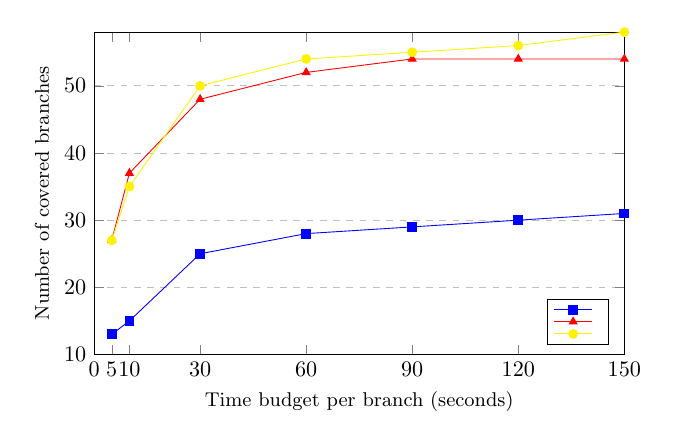
\begin{tikzpicture}[scale=0.8]
    \begin{axis}[
        xlabel={Time budget per branch (seconds)},
        ylabel={Number of covered branches},
        width=10cm,height=6.7cm,
        xmin=0, xmax=150,
        ymin=10, ymax=58,
        xtick={0,5,10,30,60,90,120,150,180},
        ytick={0,10,20,30,40,50},
        legend pos=south east,
        ymajorgrids=true,
        % xmajorgrids=true,
        grid style=dashed,
        label style={font=\small}
      ]

      \addplot[
        color=blue,
        mark=square*,
      ] coordinates {
        (5,13) (10,15) (30,25) (60,28) (90,29) (120,30) (150,31)
      };
      \addplot[
        color=red,
        mark=triangle*,
      ]  coordinates {
        (5,27) (10,37) (30,48) (60,52) (90,54) (120,54) (150,54)
      };
      \addplot[
        color=yellow,
        mark=*,
      ]   coordinates {
        (5,27) (10,35) (30,50) (60,54) (90,55) (120,56) (150,58)
      };
      \legend{$\Random$,$\Genetic$,$\RGenetic$}

    \end{axis}
  \end{tikzpicture}

  \label{fig.budget.progress}
}\\
\begin{minipage}[c]{.6\linewidth}
\subfloat[Time $t$]{
  \centering
    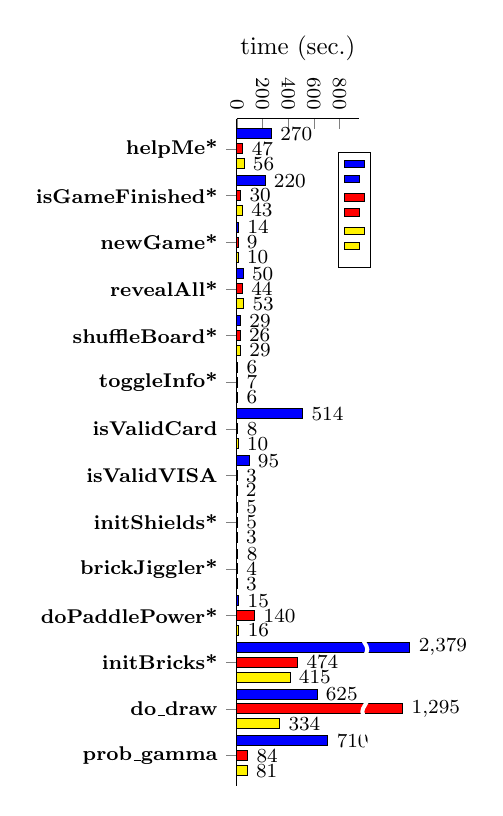
\begin{tikzpicture}[scale=0.9,rotate=-90]

    \begin{axis}[
        every axis plot post/.style={/pgf/number format/fixed},
        ybar,
        ymin=0,ymax=950,
        width=11cm,height=3.3cm,
        bar width=4pt,
        enlarge x limits=0.05,
        legend style={rotate=45,anchor=north west,font=\footnotesize,legend columns=-1,at={(0.05,1.1)}},
        legend cell align={left},
        ylabel={time (sec.)},
        symbolic x coords={helpMe*,isGameFinished*,newGame*,revealAll*,shuffleBoard*,toggleInfo*,isValidCard,isValidVISA,initShields*,brickJiggler*,doPaddlePower*,initBricks*,do\_draw,prob\_gamma},
        xtick=data,
        restrict y to domain*=0:1350, % Cut values off at 14
        visualization depends on=rawy\as\rawy, % Save the unclipped values
        after end axis/.code={ % Draw line indicating break
          \draw [ultra thick, white, decoration={snake, amplitude=1pt}, decorate] (rel axis cs:0,1.05) -- (rel axis cs:1,1.05);
        },
        nodes near coords={%
          \pgfmathprintnumber{\rawy}% Print unclipped values
        },
        every node near coord/.append style={rotate=90,anchor=west,font=\footnotesize},
        % every node near coord/.append style={font=\footnotesize},
        axis lines*=left,
        clip=false,
        x tick label style={rotate=90,anchor=east,font=\footnotesize\bfseries},
        y tick label style={font=\footnotesize}
      ]
      \addplot[fill=blue] coordinates {(helpMe*,270) (isGameFinished*,220) (newGame*,14) (revealAll*,50) (shuffleBoard*,29) (toggleInfo*,6) (isValidCard,514) (isValidVISA,95) (initShields*,5) (brickJiggler*,8) (doPaddlePower*,15)  (initBricks*,2379) (do\_draw,625) (prob\_gamma,710)};
      \addplot[fill=red] coordinates {(helpMe*,47)  (isGameFinished*,30)  (newGame*,9)  (revealAll*,44) (shuffleBoard*,26) (toggleInfo*,7) (isValidCard,8)   (isValidVISA,3)  (initShields*,5) (brickJiggler*,4) (doPaddlePower*,140) (initBricks*,474) (do\_draw,1295) (prob\_gamma,84)};
      \addplot[fill=yellow] coordinates {(helpMe*,56)  (isGameFinished*,43)  (newGame*,10) (revealAll*,53) (shuffleBoard*,29) (toggleInfo*,6) (isValidCard,10)  (isValidVISA,2)  (initShields*,3) (brickJiggler*,3) (doPaddlePower*,16) (initBricks*,415) (do\_draw,334) (prob\_gamma,81)};
      \legend{$\Random$,$\Genetic$,$\RGenetic$}
    \end{axis}
  \end{tikzpicture}

  \label{fig.gen.time.comp}
}
\end{minipage}
\hfill
\begin{minipage}[c]{.3\linewidth}
\subfloat[Speed $t/i$]{
  \centering
    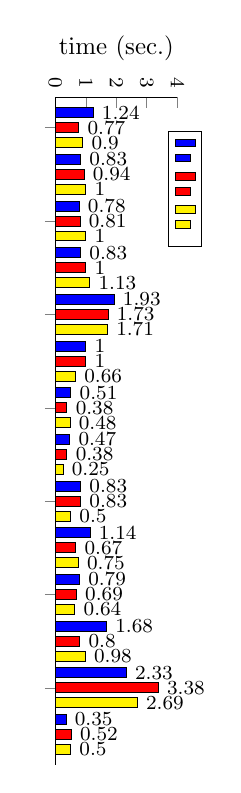
\begin{tikzpicture}[scale=0.9,rotate=-90]
    \begin{axis}[
        every axis plot post/.style={/pgf/number format/fixed},
        ybar,
        ymin=0,ymax=4,
        width=11cm,height=3.3cm,
        bar width=4pt,
        enlarge x limits=0.05,
        legend style={at={(0.05,1.2)},anchor=north west,font=\footnotesize,legend columns=-1},
        legend cell align={left},
        ylabel={time (sec.)},
        symbolic x coords={helpMe*,isGameFinished*,newGame*,revealAll*,shuffleBoard*,toggleInfo*,isValidCard,isValidVISA,initShields*,brickJiggler*,doPaddlePower*,initBricks*,do\_draw,prob\_gamma},
        %xtick=data,
        nodes near coords,
        every node near coord/.append style={rotate=90, anchor=west, font=\footnotesize},
        % every node near coord/.append style={font=\footnotesize},
        axis lines*=left,
        clip=false,
        % x tick label style={rotate=90,anchor=east,font=\footnotesize\bfseries},
        xticklabels={,,},
        y tick label style={font=\footnotesize}
      ]
      \addplot[fill=blue] coordinates {(helpMe*,1.24) (isGameFinished*,0.83) (newGame*,0.78) (revealAll*,0.83) (shuffleBoard*,1.93) (toggleInfo*,1) (isValidCard,0.51) (isValidVISA,0.47) (initShields*,0.83) (brickJiggler*,1.14) (doPaddlePower*,0.79)  (initBricks*,1.68) (do\_draw,2.33) (prob\_gamma,0.35)};
      \addplot[fill=red] coordinates {(helpMe*,0.77)  (isGameFinished*,0.94)  (newGame*,0.81)  (revealAll*,1) (shuffleBoard*,1.73) (toggleInfo*,1) (isValidCard,0.38)   (isValidVISA,0.38)  (initShields*,0.83) (brickJiggler*,0.67) (doPaddlePower*,0.69) (initBricks*,0.8) (do\_draw,3.38) (prob\_gamma,0.52)};
      \addplot[fill=yellow] coordinates {(helpMe*,0.9)  (isGameFinished*,1)  (newGame*,1) (revealAll*,1.13) (shuffleBoard*,1.71) (toggleInfo*,0.66) (isValidCard,0.48)  (isValidVISA,0.25)  (initShields*,0.5) (brickJiggler*,0.75) (doPaddlePower*,0.64) (initBricks*,0.98) (do\_draw,2.69) (prob\_gamma,0.5)};
      \legend{$\Random$,$\Genetic$,$\RGenetic$}
    \end{axis}
  \end{tikzpicture}

  \label{fig.get.cost}
}
\end{minipage}
\end{minipage}
\hfill
\begin{minipage}[c]{.55\linewidth}
\subfloat[Test Generation Summary]{
      \scriptsize
    \begin{tabular}{l|ccc|ccc|ccc|ccc|ccc}
      \toprule
      \multirow{2}{*}{\textbf{NAME}} &   \multicolumn{3}{c|}{$m_{\Random}$} & \multicolumn{3}{c|}{$m_{\Genetic}$} & \multicolumn{3}{c|}{$m_{\RGenetic}$} & \multirow{2}{*}{$\frac{t_{\Random}}{t_{\Genetic}}$} &  \multirow{2}{*}{$\frac{t_{\Random}}{t_{\RGenetic}}$} & \multirow{2}{*}{$\frac{t_{\Genetic}}{t_{\RGenetic}}$}   & \multirow{2}{*}{\hfil $_{\Genetic}^{\Random}$} &  \multirow{2}{*}{\hfil $_{\RGenetic}^{\Random}$} & \multirow{2}{*}{\hfil $_{\RGenetic}^{\Genetic}$} \\
      \cline{2-10} % \!:\!
                             & $i$      & $t$  & $t/i$     & $i$& $t$&$t/i$             &$i$ &$t$ &$t/i$               &      &       &        &      &       &      \\
      \midrule
    \textbf{helpMe}*         & 218      & 270  & 1.24      & 61 & 47 & 0.77             & 62 & 56 & 0.9                & 5.74 & 4.82  & 0.84   &      &      &       \\
    $(3,4,\inFor)$           & 4        & 4    & 1         & 5  & 3  & 0.6              & 8  & 6  & 0.75               & 1.33 & 0.67  & 0.5    & - & 0.39 & 0.37  \\
    $(5,6,\thenBr)$          & 4        & 5    & 1.25      & 8  & 6  & 0.75             & 7  & 5  & 0.71               & 0.83 & 1     & 1.2    & - & -  & -  \\
    $(5,15,\elseBr)$         & 121      & 156  & 1.29      & 24 & 21 & 0.86             & 23 & 24 & 1.04               & 7.43 & 6.5   & 0.88   & 0.87 & 0.86 & -  \\
    $(9,10,\thenBr)$         & 85       & 101  & 1.19      & 18 & 14 & 0.78             & 19 & 17 & 0.89               & 7.21 & 5.94  & 0.82   & 0.98 & 0.95 & -  \\
    $(9,14,\elseBr)$         & 4        & 4    & 1         & 6  & 4  & 0.67             & 5  & 4  & 0.8                & 1    & 1     & 1      & - & - & -  \\
    \hline
    \textbf{isGameFinished}* & 264      & 220  & 0.83      & 32 & 30 & 0.94             & 43 & 43 & 1                  & 7.33 & 5.12  & 0.7    &      &      &        \\
    $(7,8,\thenBr)$          & 37       & 30   & 0.81      & 8  & 8  & 1                & 12 & 13 & 1.08               & 3.75 & 2.31  & 0.62   & -  & 0.66 & -   \\
    $(10,11,\thenBr)$        & \un{200} & 167  & 0.84      & 11 & 10 & 0.91             & 10 & 11 & 1.1                & 16.7 & 15.18 & 0.91   & 0.88 & 0.96 & -   \\
    $(10,14,\elseBr)$        & 25       & 21   & 0.84      & 11 & 11 & 1                & 19 & 18 & 0.95               & 1.91 & 1.17  & 0.61   & - & - & -   \\
    \hline
    \textbf{newGame}*
                             & 18       & 14   & 0.78      & 11 & 9  & 0.81             & 10 & 10 & 1                  & 1.56 & 1.4   & 0.9    &      &      &      \\
    $(6,7,\thenBr)$          & 16       & 12   & 0.75      & 9  & 7  & 0.78             & 8  & 8  & 1                  & 1.71 & 1.5   & 0.88   & 0.64 & 0.65 & -  \\
    \hline
    \textbf{revealAll}*
                             & 60       & 50   & 0.83      & 44 & 44 & 1                & 47 & 53 & 1.13               & 1.14 & 0.94  & 0.83   &      &      &        \\
    $(2,3,\inFor)$           & 25       & 20   & 0.8       & 24 & 24 & 1                & 24 & 27 & 1.13               & 0.83 & 0.74  & 0.89   & - & - & -  \\
    $(4,5,\inFor)$           & 35       & 30   & 0.86      & 20 & 20 & 1                & 23 & 26 & 1.13               & 1.5  & 1.15  & 0.77   & 0.62 & -   &  0.37  \\
    \hline
    \textbf{shuffleBoard}*
                             & 15       & 29   & 1.93      & 15 & 26 & 1.73             & 17 & 29 & 1.71               & 1.12 & 1     & 0.9    &      &      &       \\
    $(13,14,\thenBr)$        & 5        & 10   & 2         & 5  & 9  & 1.8              & 6  & 10 & 1.67               & 1.11 & 1     & 0.9    & - & - & -  \\
    $(17,18,\thenBr)$        & 5        & 10   & 2         & 5  & 10 & 2                & 6  & 11 & 1.83               & 1    & 0.91  & 0.91   & - & - & -   \\
    \hline
   \textbf{toggleInfo}*      & 6        & 6    & 1         & 7  & 7 & 1                 & 9 & 6   & 0.66               & 0.86  & 1     & 1.17  &    &      &       \\
    $(6,7,\thenBr)$          & 2        & 2    & 1         & 3  & 3 & 1                 & 5 & 3   & 0.6                & 0.67  & 0.67  & 1     & 0.37 & 0.36 & -  \\
    \hline
   \textbf{isValidCard}      & 1001     & 514  & 0.51      & 21 & 8 & 0.38              & 21 & 10 & 0.48               & 64.25 & 51.4  & 0.8    &   &   &       \\
    $(3,6,\elseBr)$          & \un{200} & 103  & 0.52      & 4  & 2 & 0.5               & 4  & 2  & 0.5                & 51.5  & 51.5  & 1      & 1 & 1 & -   \\
    $(7,8,\inFor)$           & \un{200} & 103  & 0.52      & 4  & 1 & 0.25              & 4  & 2  & 0.5                & 103   & 51.5  & 0.5    & 1 & 1 & -  \\
    $(10,11,\thenBr)$        & \un{200} & 102  & 0.51      & 4  & 2 & 0.5               & 4  & 2  & 0.5                & 51    & 51    & 1      & 1 & 1 & -  \\
    $(10,13,\elseBr)$        & \un{200} & 106  & 0.53      & 4  & 1 & 0.25              & 4  & 2  & 0.5                & 106   & 53    & 0.5    & 1 & 1 & -  \\
    $(14,15,\inFor)$         & \un{200} & 100  & 0.5       & 4  & 2 & 0.5               & 4  & 2  & 0.5                & 50    & 50    & 1      & 1 & 1 & -  \\
    \hline
   \textbf{isValidVISA}      & 201      & 95   & 0.47      & 8  & 3 & 0.38              & 8  & 2  & 0.25               & 31.67 & 47.5  & 1.5    &   &   &       \\
    $(2,3,\thenBr)$          & \un{200} & 95   & 0.48      & 7  & 3 & 0.43              & 7  & 2  & 0.29               & 31.67 & 47.5  & 1.5    & 1 & 1 & -  \\
    \hline
   \textbf{initShields}*     & 6        & 5    & 0.83      & 6  & 5 & 0.83              & 6  & 3  & 0.5                & 1      & 1.67 & 1.67   &      &      &       \\
    $(2,3,\inFor)$           & 6        & 5    & 0.83      & 6  & 4 & 0.67              & 6  & 3  & 0.5                & 1.25   & 1.67 & 1.33   & 0.83 & 0.84 & -  \\
    \hline
   \textbf{brickJiggler}*    & 7        & 8    & 1.14      & 6  & 4 & 0.67              & 4  & 3  & 0.75               & 2      & 2.67 & 1.33   &      &      &       \\
    $(2,3,\thenBr)$          & 6        & 7    & 1.17      & 5  & 3 & 0.6               & 3  & 2  & 0.67               & 2.33   & 3.5  & 1.5    & 0.83 & 0.85 & -  \\
    \hline
   \textbf{doPaddlePower}*   & 19       & 15   & 0.79      & 204  & 140 & 0.69          & 25 & 16  & 0.64              & 0.11   & 0.94 & 8.75   &       &      &      \\
    $(10,11,\thenBr)$        & 16       & 12   & 0.75      & \un{200} & 136 & 0.68      & 22 & 13  & 0.59              & 0.09   & 0.92 & 10.46  &  0.02 & - & 0.94 \\
   \midrule
    \textbf{TOTAL (simple)}          & 1816      & 1226 & 0.68      & 415 & 323 & 0.78          & 252 & 231 & 0.92              & 3.8    & 5.31  & 1.4       &   &   &    \\
    \bottomrule
   \textbf{initBricks}*      & 1418     & 2379 & 1.68      & 593  & 474 & 0.8           & 422 & 415 & 0.98             & 5.02   & 5.73  & 1.14   &      &      &       \\
    $(6,7,\thenBr)$          & 2        & 3    & 1.5       & 5    & 4   & 0.8           & 3   & 3   & 1                & 0.75   & 1     & 1.33   & - & -  & -   \\
    $(6,10,\elseBr)$         & 15       & 23   & 1.53      & 6    & 6   & 1             & 6   & 6   & 1                & 3.83   & 3.83  & 1      & 0.87 & 0.83 & -   \\
    $(11,12,\thenBr)$        & \un{200} & 317  & 1.59      & 14   & 12  & 0.86          & 17  & 15  & 0.88             & 26.41  & 21.13 & 0.8    & 0.93 & 0.91 & -  \\
    $(11,15,\elseBr)$        & 18       & 30   & 1.67      & 6    & 6   & 1             & 6   & 6   & 1                & 5      & 5     & 1      & 0.89 & 0.86 & -  \\
    $(16,17,\thenBr)$        & \un{200} & 324  & 1.62      & 17   & 14  & 0.82          & 17  & 16  & 0.94             & 23.14  & 20.25 & 0.88   & 0.96 & 0.96 & -  \\
    $(16,20,\elseBr)$        & 25       & 40   & 1.6       & 7    & 7   & 1             & 8   & 7   & 0.88             & 5.71   & 5.71  & 1      & 0.89 & 0.86 & -  \\
    $(21,22,\thenBr)$        & \un{200} & 310  & 1.55      & 14   & 13  & 0.93          & 17  & 17  & 1                & 23.85  & 18.24 & 0.76   & 0.94 & 0.9  & 0.36  \\
    $(21,25,\elseBr)$        & 26       & 41   & 1.58      & 7    & 7   & 1             & 8   & 7   & 0.88             & 5.86   & 5.86  & 1      & 0.94 & 0.87 & -  \\
    $(29,30,\thenBr)$        & \un{200} & 330  & 1.65      & 66   & 58  & 0.88          & 74  & 70  & 0.95             & 5.69   & 4.71  & 0.83   & 0.82 & 0.88 & -   \\
    $(29,37,\elseBr)$        & 2        & 4    & 2         & 3    & 3   & 1             & 3   & 4   & 1.33             & 1.33   & 1     & 0.75   & - & - & -  \\
    $(38,39,\thenBr)$        & 185      & 328  & 1.77      & 85   & 67  & 0.79          & 48  & 44  & 0.92             & 4.9    & 7.45  & 1.52   & 0.87 & 0.88 & -  \\
    $(38,46,\elseBr)$        & 2        & 4    & 2         & 3    & 4   & 1.33          & 3   & 4   & 1.33             & 1      & 1     & 1      & 0.64 & - & -  \\
    $(47,48,\thenBr)$        & 187      & 336  & 1.8       & \un{200} & 141 & 0.7       & 127 & 131 & 1.03             & 2.38   & 2.56  & 1.08   & 0.8  & 0.8  & -  \\
    $(47,55,\elseBr)$        & 2        & 4    & 2         & 3    & 3   & 1             & 3   & 4   & 1.33             & 1.33   & 1     & 0.75   & 0.66 & 0.61 & -  \\
    $(56,57,\thenBr)$        & 109      & 198  & 1.82      & 50   & 43  & 0.86          & 49  & 47  & 0.96             & 4.6    & 4.21  & 0.91   & 0.76 & 0.75 & -   \\
    $(56,64,\elseBr)$        & 2        & 4    & 2         & 3    & 3   & 1             & 3   & 4   & 1.33             & 1.33   & 1     & 0.75   & 0.64 & 0.61 & -  \\
    $(69,70,\thenBr)$        & 2        & 4    & 2         & 3    & 4   & 1.33          & 3   & 4   & 1.33             & 1      & 1     & 1      & - & - & -  \\
    $(69,71,\elseBr)$        & 41       & 81   & 1.98      & 95   & 84  & 0.88          & 27  & 26  & 0.96             & 0.96   & 3.12  & 3.23   & - & 0.68 & 0.61  \\
    \hline
    \textbf{do\_draw}        & 268      & 625  & 2.33      & 383  & 1295 & 3.38         & 124 & 334 & 2.69             & 0.48   & 1.87  & 3.88   &      &      &       \\
    $(6,7,\thenBr)$          & 8        & 19   & 2.38      & 6    & 25   & 4.1          & 7   & 20  & 2.86             & 0.76   & 0.95  & 1.25   & - & -  &  0.62 \\
    $(8,9,\thenBr)$          & 10       & 23   & 2.3       & 6    & 17   & 2.83         & 7   & 21  & 3                & 1.35   & 1.1   & 0.81   & 0.63 & 0.62 &  - \\
    $(8,11,\elseBr)$         & 144      & 343  & 2.39      & 17   & 51   & 3            & 19  & 57  & 3                & 6.73   & 6.02  & 0.89   & 0.91 & 0.91 &  - \\
    $(44,45,\thenBr)$        & 57       & 144  & 2.5       & \un{200} & 681  & 3.4      & 40  & 111 & 2.78             & 0.21   & 1.3   & 6.14   & 0.16 & - &  0.89 \\
    $(48,49,\thenBr)$        & 26       & 68   & 2.61      & 137  & 492  & 3.59         & 34  & 97  & 2.85             & 0.14   & 0.7   & 5.07   & 0.24 & - &  0.74 \\
    \hline
    \textbf{prob\_gamma}     & 2006     & 710  & 0.35      & 163 & 84   & 0.52          & 162 & 81  & 0.5              & 8.45   & 8.77  & 1.04   &  &   &        \\
    $(4,5,\thenBr)$          & \un{200} & 71   & 0.36      & 2   & 1    & 0.5           & 2   & 1   & 0.5              & 71     & 71    & 1      & 1 & 1 &  -  \\
    $(6,7,\thenBr)$          & \un{200} & 71   & 0.36      & 2   & 1    & 0.5           & 2   & 1   & 0.5              & 71     & 71    & 1      & 1 & 1 &  -  \\
    $(6,9,\elseBr)$          & \un{200} & 70   & 0.35      & 2   & 1    & 0.5           & 2   & 1   & 0.5              & 70     & 70    & 1      & 1 & 1 &  -  \\
    $(10,11,\thenBr)$        & \un{200} & 72   & 0.36      & 62  & 42   & 0.68          & 61  & 40  & 0.66             & 1.71   & 1.8   & 1.05   & 1 & 1 &  -  \\
    $(10,13,\elseBr)$        & \un{200} & 71   & 0.36      & 2   & 1    & 0.5           & 2   & 1   & 0.5              & 71     & 71    & 1      & 1 & 1 &  -  \\
    $(16,17,\inWhile)$       & \un{200} & 70   & 0.35      & 2   & 1    & 0.5           & 2   & 1   & 0.5              & 70     & 70    & 1      & 1 & 1 &  -  \\
    $(20,21,\thenBr)$        & \un{200} & 70   & 0.35      & 6   & 2    & 0.33          & 6   & 3   & 0.5              & 35     & 23.33 & 0.67   & 1 & 1 &  -  \\
    $(20,23,\elseBr)$        & \un{200} & 72   & 0.36      & 2   & 1    & 0.5           & 2   & 1   & 0.5              & 72     & 72    & 1      & 1 & 1 &  -  \\
    $(30,31,\thenBr)$        & \un{200} & 72   & 0.36      & 53  & 23   & 0.43          & 52  & 22  & 0.42             & 3.13   & 3.27  & 1.05   & 1 & 1 &  -  \\
    $(34,35,\thenBr)$        & \un{200} & 72   & 0.36      & 24  & 10   & 0.42          & 25  & 10  & 0.4              & 7.2    & 7.2   & 1      & 1 & 1 &  -  \\
    \midrule
    \textbf{TOTAL (diff.)}           & 3692     & 3714 & 1         & 1139 & 1853 & 1.63         & 708 & 830 & 1.17             & 2      & 4.47  & 2.23   &   &   &    \\
    %% \midrule
    %% \midrule
    \bottomrule
    \bottomrule
    \textbf{TOTAL (global)} & 5507      & 4940 & 0.9       & 1554 & 2176 & 1.4          & 966 & 1061 & 1.1             & 2.27   & 4.66  & 2.05       &   &   &    \\
    \bottomrule
    \end{tabular}


  \label{tbl.stats}
}
\end{minipage}
\caption{Statistics of experimental results for $\Random$, $\Genetic$ and $\RGenetic$ (time $t$ is in seconds; \underline{200} indicates branch is not covered; (-) means the data is insignificant).}
\label{lab3}
\end{figure*}


\subsection{Results}
\label{sub.sec.eval.results}

To study the effectiveness and efficiency of our test generation framework, we exercised each algorithm ($\Random$, $\Genetic$ and $\RGenetic$) against all branches of the functions in Table~\ref{tbl.case.studies}. Due to the probabilistic nature of the test generation process~\cite{arcuri2011practical}, the experiments have been repeated 50 times to achieve statistical significance. Table~\ref{tbl.stats} summarizes the evaluation results. For each algorithm, we computed the following \emph{medians} per branch: the number of iterations~($i$), time in seconds~($t$), and their ratio~($t/i$). In the table, these values are grouped into three columns $m_{\Random}$, $m_{\Genetic}$ and $m_{\RGenetic}$ one for each algorithm. The next group of columns $t_{\Random}/t_{\Genetic}$, $t_{\Random}/t_{\RGenetic}$ and $t_{\Genetic}/t_{\RGenetic}$ presents the relative performance of each pair of the testing algorithm $(\Random,\Genetic)$, $(\Random,\RGenetic)$, and $(\Genetic,\RGenetic)$ respectively. To the right of the function name, we also present accumulated statistics\footnote{because of the missing branches, the function's summary may not be equal to the sum of the branches, e.g. see the \emph{toggleInfo} function}.

According to the industry standard~\cite{bray1997c4}, functions with a CC below 10 are considered as easy to test, and above 10 are reasonably challenging. We call the functions of the first type ``simple'', and ``difficult'' otherwise. The three functions \mbox{\emph{initBricks}}, \emph{do_draw} and \emph{prob_gamma} at the bottom of Table~\ref{tbl.case.studies} are difficult with CC's of 13, 14 and 16 respectively. Table~\ref{tbl.stats.sum} summarizes the results of the experiment such as coverage, execution time per branch and significance.

\textbf{RQ1 (effectiveness)}: To answer this question, we measure the branch coverage achieved by each test generation algorithm. Given a fixed limit on the number of test iterations, 200 in our case, a search algorithm cannot guarantee finding a solution. The underlined values in Table~\ref{tbl.stats} like $\underline{200}$ indicate branches which were not covered by the respective algorithms. The main reason for the random generation~($\Random$) to fail is the large size of the search space and the lack of any feedback in the generation process, e.g. branch $(10,11)$ of the \emph{isGameFinished} function. In the case of the genetic approach~($\Genetic$), it  may get stuck at a plateau because the fitness function does not provide sufficient guidance, whereas $\Random$ could still escape the plateau by sheer luck. We encountered three such cases in our study: branches $(10,11)$, $(47,48)$ and $(45,45)$ of the function \emph{doPaddlePower}, \emph{initBricks} and \emph{do_draw}, respectively. They motivated us to introduce the GA with restart ($\RGenetic$) which combines the strengths of both $\Random$ and $\Genetic$. It leverages the genetic search while the fitness continues to improve, and restarts the search with a new target, when the fitness suboptimally converges. As our evaluation has shown, $\RGenetic$ not only managed to outperform $\Random$ and cover the three problematic branches above, but it has generally improved the results of $\Genetic$, e.g. branch $(69,71)$ of the \emph{initBricks} function.\\
\framebox{
  \parbox[t][1.1cm]{0.95\linewidth}{
    Across all subjects, the $\RGenetic$ algorithm achieved 100\% branch coverage, with $\Genetic$ in the second place with 95\% coverage, and, finally, $\Random$ with  63\% coverage.
  }
}

Additionally, we have investigated how the coverage progresses with the change of time budget assigned per branch. This experiment models different time dependent testing scenarios, used in practice. E.g. running tests inside an IDE should be fast; as part of the continuous integration we may afford a longer waiting time; and regression testing over night may take hours. Figure~\ref{fig.budget.progress} illustrates the progress of the algorithms across budget categories from 5 to 150 seconds per branch. Random test generation consistently underperforms the genetic one across all budget categories by at least a factor of two. Eventually, it converges around 52\% coverage. Given 5 seconds per branch, both $\Genetic$ and $\RGenetic$ perform equally at the rate of 45\%. When the budget increases towards 10 seconds, $\Genetic$ slightly outperforms $\RGenetic$, 60\% against 63\% respectively. But when the budget rises to 30 seconds, $\RGenetic$ overtakes $\Genetic$ and the distance between them continues growing further with the budget increase (starting from 120 seconds).\\
\framebox{
  \parbox[t][0.7cm]{0.95\linewidth}{
We suggest to use $\Genetic$ for rapid testing during development, and later in integration testing switch to $\RGenetic$.
  }
}

\textbf{RQ2 (efficiency):} To answer this question, we compare the actual execution time of our test generation algorithms. The bar chart in Figure~\ref{fig.gen.time.comp} illustrates how the median coverage time differs for each algorithm at the function level. There are two cases, \emph{revealAll} and \emph{doPaddlePower} out of 14, where $\Random$ just slightly outperformed $\RGenetic$ by 6\%, and two more cases \emph{shuffleBoard} and \emph{toggleInfo}, where they performed equally. In all other cases, $\RGenetic$ significantly outperformed $\Random$ by minimum of 40\%~(\emph{newGame}) and a maximum of 510\%~(\emph{isValidCard}).

Looking separately at the average execution time for \emph{simple} and \emph{difficult} functions in Table~\ref{tbl.stats.sum}, we conclude that $\RGenetic$ was the fastest algorithm in both cases with  7 and 25 seconds per branch. For simple functions, the performance of $\Genetic$ was quite close to $\RGenetic$, only 9 seconds, but for difficult functions it was two times slower. In all categories, $\Random$ was much slower than both genetic alternatives.\\
\framebox{
  \parbox[t][0.7cm]{0.95\linewidth}{
    $\RGenetic$ outperformed both $\Genetic$ and $\Random$ with an average execution time per branch of 19, 39 and 88 seconds, respectively.
  }
}

Another question related to the efficiency is the computational cost of one iteration of each algorithm. It is useful to know in order to choose the generation limit. The cost, shown in column $t/i$ in Table~\ref{tbl.stats}, is calculated as the relation between the execution time and the number of generations, i.e. it measures the speed of one iteration. Figure~\ref{fig.get.cost} presents the cost comparison for all three algorithms in our study. Among the factors impacting the iteration cost are the population size (50 candidates in our case) and the fitness evaluation of one candidate. The length of an execution trace correlates with the fitness evaluation. So, an exceptional program termination leads to short traces, whereas loops tend to produce longer traces. For example, the \emph{do_draw} function has long traces because it only operates with the primitive types thus never rises exceptions, and at the same time, it consists of 40 LOC. In our evaluation, the iteration cost varied between 0.25 and 3.59 seconds.\\
\framebox{
  \parbox[t][0.7cm]{0.95\linewidth}{
    On average, one algorithm iteration took one second for $\Random$ and $\RGenetic$, $\Genetic$ performed somewhat worse at 1.4 seconds.
  }
}

\textbf{RQ3 (significance):} Our testing framework is randomized by nature, therefore we need to conduct a statistical analysis to assess the \emph{significance} and \emph{effect size} of our results. This analysis is based on 50 executions produced by each test algorithm $\Random$, $\Genetic$ and $\RGenetic$. Following recommendations on the assessment of randomized algorithms~\cite{arcuri2011practical}, we use the non-parametric Mann-Whitney U-test~\cite{mann1947test} and the Vargha-Delaney $\hat{A}_{12}$ statistics~\cite{vargha2000critique} for measuring statistical significance ($\alpha=0.05$) and effect size, respectively. In Table~\ref{tbl.stats} the three columns to the right show the $\hat{A}_{12}$ values for all algorithm combinations, where this value is significant and '-' otherwise. Thus, the higher the value in the $_{\Genetic}^{\Random}$ column, indicates that $\Random$ is slower in comparison with $\Genetic$. Depending on the actual $\hat{A}_{12}$ value, the effect size can be small (0.56), medium (0.64), and large (0.71).\\
\framebox{
  \parbox[t][0.65cm]{0.95\linewidth}{
    Both $\Genetic$ and $\RGenetic$ largely outperform $\Random$ in 50\% cases generally across the board and 67\% on the difficult functions.
  }
}

\textbf{RQ4 (comparison):} We evaluate \Confix~\cite{amin:ase15} as the only available alternative for the generation of DOM fixtures. The authors suggest that \Confix\ achieves higher branch and statement coverage by being combined with \Jalangi~\cite{sen2013jalangi} --- a concolic test generation tool for JS --- which is able to produce test inputs for JS arguments of primitive types. However, the available online implementation of \Confix~\cite{confixgit} has no actual integration with \Jalangi. Thus we have to fall back on plain \Confix test generation.

Experimental results are presented in Figure~\ref{tbl.confix.compare}. We report both \emph{weak} (reach the target branch) and \emph{strong} (reach the branch and terminate normally) coverage. \Confix test generation is guided by the weak coverage in contrast with the strong coverage of \Jedi. In all experimental subjects except one (\jsID{isGameFinished}), \Confix poorly performs simply due to an inability to produce appropriate input arguments. However, in the case of \jsID{isGameFinished}, which requires no inputs, it still fails to reach deeply nested branches because of imprecise symbolic representation. In particular, it cannot interpret the expression on line~\ref{isGameFinished.if1.begin} in Figure~\ref{code.isGameFinished}:
%% following expression:
\begin{center}
\begin{lstlisting}[style=htmlcssjs,language=JavaScript,basicstyle={\footnotesize\ttfamily},backgroundcolor=\color{white},frame=none,numbers=none,xleftmargin={0.2cm}]
subDivs[no].className.indexOf('sudokuSquare') >= 0
\end{lstlisting}
\end{center}
This is not a principal constraint, but to be fully addressed, \Confix should model an extensive library of built-in JS functions. \Jedi mitigates this constraint by substituting observed string literals as conceivable class names, which are additionally evolved thanks to crossover and mutation operators. We admit, however, that some constructs, e.g. jQuery, are supported by Confix but not by Jedi.\\
\framebox{
  \parbox[t][1.5cm]{0.95\linewidth}{
In a nutshell, the choice between a concolic and search-based approach is a trade-off between a labour-intensive modelling effort and long execution time, respectively, where both can reinforce each other.
  }
}

\textbf{Threats to Validity:}
The \emph{construct validity} threat is due to the choice of measurements: branch coverage and execution time. Although, the branch coverage is a common criterion used in practice, the fault finding capability is a stronger indication of testing adequacy. Reaching a target branch is only part of the problem: we also need an oracle to discriminate the program's output. In this paper, we rely on so called ``natural'' oracles such as exceptions.
%Using a stronger oracle for validation is future work.
Another practical aspect of the test generation is the test case size, since it can both complicate the readability and increase the execution time. To mitigate this issue we configured the GA to start evolution with the candidates of small sizes, which helps to prevent data explosion. Additional measure that could be applied is a minimization procedure, aka \emph{hierarchical delta debugging}~\cite{misherghi2006hdd} and its variations~\cite{herfert2017automatically}, to the GA result.

Initial GA configuration introduces a threat to the \emph{internal validity} of our empirical evaluation. The parameters we used are quite standard for similar SBST frameworks, e.g. EvoSuite. Although, not reported in the paper, we did perform a preliminary assessment of various GA configurations, which confirmed our final decision.

The threat of \emph{conclusion validity} can be affected by the stochastic nature. This risk was addressed by repeating the experiment of GA 50 times and performing a statistical analysis of the significance and effect size. We used the confidence level of 95\% measured by the Vargha-Delaney statistic and Mann-Whitney U-test.

The \emph{external validity} deals with the threat of generalization of our results due to the manual selection of the experimental subjects. To mitigate this fact, we selected the subjects either from previous  related research or found in open source. Of course, those subjects still have to meet the constraints of our testing approach. So, further research is required both to increase the power of our framework and extend the validation set.
